\section{The M Dwarf Spectral Class}
Type M dwarfs were a part of the original Draper Catalogue of Stellar Spectra \citep{Pickering90}, 
classified as having weak but non-zero hydrogen absorption features in their spectra.
The system was alphabetical: they were classified between K and O stars, 
the former having stronger hydrogen absorption and the latter none at all.
With the development of the Harvard system, \citet{Cannon01} preserved the M spectral class and placed it
at one end of the classification system, next to K stars.
We now know that M and O stars have little hydrogen absorption in their atmospheres for very different reasons
and the modern classification system maps stellar effective temperature: M dwarfs are the coolest main-sequence
stars and the least massive hydrogen burning stars in the galaxy.
Today, the boundary between K and M dwarfs is defined by the presence of titanium oxide (TiO) bands in the
atmospheres of M dwarfs \citep{Kuiper38, Morgan38}, which can form when a star's effective temperature is below approximately 3500 K.

Often, we consider M dwarfs as a single, monolithic block.
This view overlooks the incredible diversity in M dwarf physics.
The M dwarf class spans an order of magnitude in mass, 
an order of magnitude in radius, and
a factor of 40 in luminosity \citep{Veeder74}.
There are significant changes in the structure of the stars across this class as well.
Below approximately 0.35 \msun, M dwarfs become fully convective, leading to a
rapid decrease in the radius and luminosity of stars just below this boundary \citep{Chabrier97}.

At the late edge of the M dwarf class are brown dwarfs, objects without high enough central densities to 
fuse hydrogen. 
As a brown dwarf leaves the T Tauri stage of stellar evolution it has a temperature of approximately 3000 K
and a spectrum consistent with that of a mid-M dwarf.
Brown dwarfs then cool and evolve into ``late-type'' L, T, and eventually Y dwarfs at a rate 
which depends on their mass.
I will discuss the evolution of brown dwarfs more fully in Section \ref{sec:BDs}.




We can contrast the diversity in M dwarfs with the uniformity in Sunlike stars. 
The Sun has a radiative core, in which nuclear reactions are dominated by the p-p chain, and a convective 
outer layer, which contributes to the existence of a magnetic field.
The same is true for all main-sequence stars from the middle of the F spectral class through early M dwarfs: 
in terms of their structure, F7 and K3 
dwarfs have more in common than M0 and M9 dwarfs.
If the abundance of M dwarfs and the diversity of their structure had been understood at the time of the development 
of the Harvard stellar classification system, it is possible that these stars would have been awarded more than a 
single spectral type.


\section{M Dwarfs: The Silent Majority}
The first spectrum of an M dwarf was obtained only 100 years ago when 
\citet{Adams13} collected an observation of the M+M binary Groombridge 34.\footnote{The
Draper catalogue was first published in 1890 and the
Harvard stellar classification scheme in 1901. 
All of the early work in stellar spectroscopic classification of M dwarfs is based on
spectroscopy of M giants: there were no main sequence stars used to create the stellar class in which 
75\% of main sequence stars reside.}

The oldest known surviving diagram plotting stellar absolute magnitude against spectral type \citep{Russell14}, now known as a Hertsprung-Russell Diagram, includes hundreds of stars, as shown in Figure \ref{fig:HR}.
Today we know that M dwarfs make up approximately 75\% of the stars in the galaxy,
yet only $\sim$5\% of the stars included in Russell's figure are listed as
spectral type M.



\begin{figure}[hbt!]
\centering
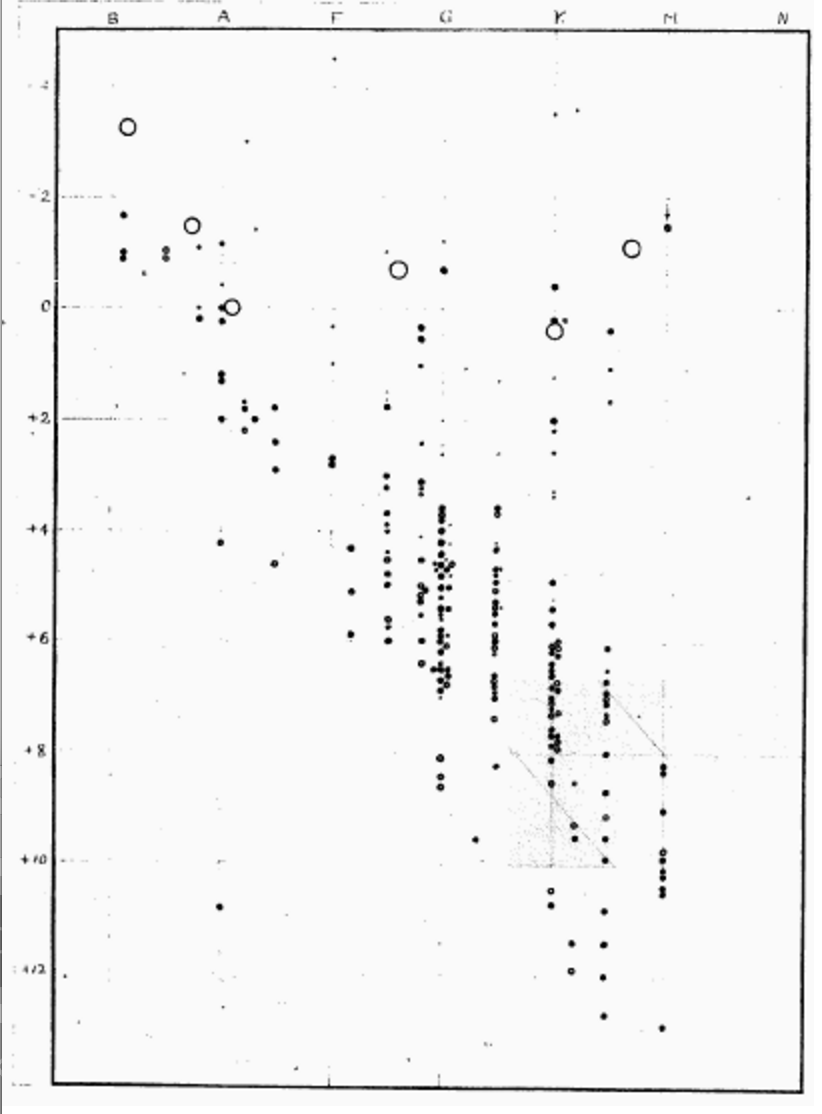
\includegraphics[width=.5\textwidth]{chapter1/hr.png}
\caption[Russell's original H-R Diagram]{The original H-R diagram, as published by
\citet{Russell14}. On the $y$-axis is absolute magnitude, equivalent to the logarithm
of the star's luminosity. On the $x$-axis is stellar spectral type, which we now know
maps approximately to stellar effective temperature.}
\label{fig:HR}
\end{figure}

The lack of M dwarfs included in these early studies stems from the physics
of M dwarfs themselves, specifically the stellar mass-luminosity relation.
To show this, let us begin with the equations of stellar structure.
The first of these declares a star is in hydrostatic equilibrium:
\begin{equation}
\frac{\d P(r)}{\d r} = - \frac{ G m \rho}{r^2 },
\label{eq:hydro}
\end{equation}
where $P(r)$ is the pressure exerted on a particle at a radius $r$, $G$ is Newton's
constant, $m$ the mass enclosed inside the radius $r$, and $\rho$ the stellar density,
itself a function of radius as well.

The second equation defines mass conservation:
\begin{equation}
\frac{\d m(r)}{\d r} = 4 \pi r^2 \rho,
\end{equation}
where $\pi$ is the ratio of a circle's circumference to its diameter,
and all other variables retain their meaning from Equation \ref{eq:hydro}.

The third equation defines energy transport:
\begin{equation}
\frac{\d L(r)}{\d r} = 4 \pi r^2 \rho \epsilon,
\end{equation}
where $L$ is the energy leaving a spherical shell of radius $r$, produced by the
material in the star interior to $r$ and $\epsilon$ is the energy released per unit
mass per second inside the star.

The final equation defines the temperature gradient inside a star. 
The exact form of this equation depends on the method for which energy is transported
inside the star.
For radiative transport, the temperature gradient is
\begin{equation}
\frac{\d T}{\d r} = - \frac{3}{4ac} \frac{\bar{\kappa} \rho}{T^3} \frac{L}{4\pi r^2}.
\end{equation}
Here, $T$ is the temperature of the star at a radius $r$, $ac$ is the radiation constant multiplied by the speed of light, also equal to four times the Stefan-Boltzmann
constant, and $\bar{\kappa}$ the mean opacity of the material.

Very low-mass stars are fully convective, not radiative, and therefore follow
a different limit:
\begin{equation}
\frac{\d T}{\d r} =  \bigg( 1 - \frac{1}{\gamma}\bigg)\frac{T}{P}\frac{\d P(r)}{\d r},
\end{equation}
where $\gamma$ is the adiabatic index, and is $5/3$ for a monatomic ideal gas,
and all other terms retain their previous meaning.

Let us consider two other proportionalities. First, we assume that the energy generation rate
inside a star is a function of its temperature and density:
\begin{equation}
\epsilon = \epsilon_0 \rho T^\nu
\end{equation}
where $\nu$ depends on the particular fusion pathway that is dominant in the core of
the star.
Second, we assume that the ideal gas law holds:
\begin{equation}
P \propto \rho T.
\end{equation}

With these six equations, we can develop a series of homology relations. We can create
a series of five linear equations with five unknown parameters: $\log T$, $\log P$, 
$\log R$, $\log \rho$, and $\log M$.
Ignoring constant terms and considering only the adiabatic case (as for fully 
convective stars),
\begin{align}
\log P &= 2 \log M - 4 \log R \nonumber \\
\log \rho &= \log M - 3 \log R \nonumber \\
\log P &= \gamma \log \rho \\
\log T &= \bigg(\frac{\gamma - 1}{\gamma}\bigg) \log P \nonumber \\
\log L &= \log \rho + \nu \log T + \log M \nonumber.
\end{align}
We can rearrange these to solve for $\log M$, finding
\begin{equation}
\log R = \bigg(\frac{2-\gamma}{4 - 3\gamma}\bigg) \log M,
\end{equation}
which we can then insert into the final equation in Equation 1.8.
This manipulation yields
\begin{equation}
\log L = \bigg(\frac{2(\nu + 1) - \gamma(2\nu + 3)}{4 - 3\gamma}\bigg) \log M,
\end{equation}
which if we consider the case where we have an ideal, fully ionized gas so that $\gamma = 5/3$ and energy generation dominated by the p-p chain so that $\nu = 4$, we find
\begin{equation}
\log L \approx 8.33 \log M
\end{equation}
or $L \propto M^{8.33}$! Thus, if we decrease the mass of a fully convective star by a factor of two, 
we also decrease its luminosity by a factor of 320!\footnote{The same manipulation,
considering the case of radiative transport, leads to the relation $L~\propto~M^{5.5}$,
similar to what is observed for Sunlike stars.} 

Even worse for optical observing,
the peak of the SED of a typical 3,000 K M dwarf peaks at 1 micron, well into the infrared, making them even fainter in the optical.
Even though M dwarfs make up 70\% of the nearest stars, with 250 of them located within
10 pc of the Sun \citep[e.g.][]{Henry06}, there are no M dwarfs visible to the naked 
eye.
The brighest, HIP\,105090, is only $3.95 \pm 0.01$ pc from the Sun, yet has an apparent V-band magnitude of 6.76 \citep{vanLeeuwen07}.
With so many bright solar-type stars in the solar neighborhood, it is easy to understand why M dwarfs have been and often continue to be overlooked in planet search
surveys. 

\section{Radial Velocity Planet Searches}
\subsection{Stellar Radial Velocities}
Planets do not orbit their host stars.
Planets and stars, like any pair of bodies orbiting each other, orbit their common
center of mass, or barycenter.
For circular orbits, the planet and star velocities are constant, and the observed
radial component of the velocity is modulated sinusoidally with the period of the planet
as the velocity vector changes direction.
The magnitude of the RV signal in this case depends only the mass of the planet, $m$, 
the mass of the star, $M$, the orbital period, $P$, and the unknown inclination $i$.
Specifically, by taking the time derivative of the position of the star in time,
the RV can be shown to be
\begin{equation}
v_r = \bigg(\frac{2\pi G}{P}\bigg)^{1/3} \frac{m \sin i}{(M+m)^{2/3}} \cos{\nu}.
\end{equation}
Here, $G$ is Newton's constant and $\nu$ the mean anomaly of the planet, which in the circular case increases
linearly from $0$ to $2\pi$ in time over the course of one orbit.
For Jupiter, the Sun's reflex RV motion is 13 m s$^{-1}$; for Earth, 9 cm s$^{-1}$.
We see that the velocity depends on the mass ratio between the planet and star, meaning
that we can only characterize the planet as well as we understand the star.

For planets on eccentric orbits, the math is more complicated.
Again, the derivation begins with the time derivative of the position of the star, but
in the eccentric case neither the linear or angular velocity is constant \citep{Kepler09}.
It can be shown that the radial velocity equation becomes
\begin{equation}
v_r = \bigg(\frac{2\pi G}{P}\bigg)^{1/3} \frac{m \sin i}{(M+m)^{2/3}} \frac{1}{\sqrt{1-e^2}}
(e \cos \omega + \cos(\omega + \nu)),
\label{eq:rv}
\end{equation}
where $e$ is the eccentricity and $\omega$ the argument of periapse, the angle relative
to the plane of the sky at which the planet and star make their closest approach.
All other terms retain their previous meaning, but from Kepler's second law, the true anomaly 
no longer increases linearly in time.
While we can easily measure the expected RV of the star at any position in its 
orbit, we do not know the time at which the star will be at that position.

To calculate the expected RV at a given time, we invoke the mean anomaly, which represents the mean angular motion of the 
two bodies. 
It is defined to be zero at the time of periapse, $\tau$, and at all other times $t$ can 
be calculated such that
\begin{equation}
M = \frac{2\pi}{P}(t-\tau).
\end{equation}
It therefore increases linearly in time from 0 to $2\pi$.
The true anomaly can be calculated from the mean anomaly through the eccentric anomaly, 
$E$, such that
\begin{equation}
M = E - e \sin E.
\end{equation}
This is a transcendental equation and requires an approximate numerical solution.
Once the eccentric anomaly is determined, the true anomaly can be determined as well,
such that
\begin{equation}
\tan \frac{\nu}{2} = \sqrt{\frac{1+e}{1-e}} \tan \frac{E}{2}.
\end{equation}
With that, we can solve Equation \ref{eq:rv} and measure the RV of a star at any time.
We note that all three anomalies are identical in the circular case.

Of course, we can only use these equations if we can measure variations in the stellar RV
itself.
Fortunately, we can leverage stellar atmospheres for this purpose.
Stars with masses below $\approx 1.3$ \msun\ have convective outer layers, generating
magnetic activity which provides a torque as charged particles escape their 
host star along magnetic
field lines \citep{Shu94}.
The spin-down is a predictable function of the star's mass and age, leading to the use
of rotation rates as a probe of stellar ages \citep{Barnes03}.
G dwarfs at the age of the Sun rotate at only 1 km s$^{-1}$ at their equators.
With a full spectrum of spectral lines to consider, the RV of the star can be 
measured to 2-5 m s$^{-1}$ depending on the instrument.
At this level, systematic effects induced by the instrument can dominate over any planetary
signal: in the typical mode used for planet searches,
the resolution of Keck/HIRES is 48,000, leading to a pixel scale of 6.2 km s$^{-1}$ pixel$^{-1}$.
To combat this, one of two approaches are taken.
At Keck/HIRES, observers place an iodine cell in the light path before the starlight
enters the instrument itself \citep{Butler96}.
Iodine has many absorption features in the optical with precisely known wavelengths,
so the cell creates a precise, stable wavelength scale to compare against the stellar
signal. 
The iodine also provides information about the shape of the instrumental profile during
each observation.
At other telescopes, including HARPS, the spectrograph slit is replaced with a fiber,
and the instrument is placed in a temperature and pressure controlled enclosure, so that
the environment or motion of the telescope does not affect the wavelength zeropoint or
instrumental profile.


\subsection{History of RV Searches}
The first radial velocity (RV) planet searches focused almost exclusively on Sunlike
(FGK) stars, a reasonable choice as these are the brightest main sequence stars for 
which magnetic braking occurs, leading to slow rotation.

The first planet detected around a main sequence star other than the Sun was discovered
in 1995 with the detection of 51\,Pegasi\,b, a planet with an orbital period of 4.23 days
and a mass of $0.472 \pm 0.039$ \mjup\ \citep{Mayor95}.
Quickly, dozens of similar ``hot Jupiter'' planets with masses larger than Saturn but 
periods around three days were discovered \citep[e.g.][]{Butler97, Marcy98, Wright07}.

As more planets were detected around FGK dwarfs, surveys expanded to include other
types of stars.
As stated previously, A stars do not make ideal RV survey targets due to their rapid
rotation.
However, when these stars evolve off the main sequence onto the subgiant branch,
conservation of angular momentum results in a large increase in the rotation period and
thus a decrease in $v \sin i$, making these stars amenable to RV planet searches.
These ``Retired A stars'' were found to have fewer hot Jupiters than their less massive
counterparts, but a higher giant planet occurrence rate overall \citep{Johnson07b,
Bowler10, Johnson11b}.

M dwarfs have many narrow spectral features and make ideal planet search targets as
long as they are near enough to be observable.
Nearly immediately, researchers detected giant planets around M dwarfs \citep{Butler04, Butler06}, but the occurrence rate of giant planets around M dwarfs was found to be 
considerably lower than around higher mass stars.
Only $\approx 3\%$ of M dwarfs host a planet at least as massive as Jupiter 
within 2.5 AU \citep{Johnson10a, Bonfils13}.
These surveys also showed a correlation between giant planet occurrence and stellar
metallicity \citep{Fischer05, JohnsonApps09}.



To date nearly 600 planets have been discovered via RV variations.
These results show hot Jupiters orbit approximately 1\% of Sunlike stars \citep{Wright12}.
They also show that 10\% of systems have a Saturn-mass or larger planet with orbital periods
shorter than 2000 days \citep{Cumming08}.
By extrapolating the observed distribution outward, the same authors predict 20\% of FGK dwarfs host a gas giant planet within 20 AU.

Despite the large numbers of planets detected so far, RV surveys have substantial
limitations.
There has been substantial work on improving RV precision, both
in instrument development and in understanding stellar activity \citep{Fischer16}.
Yet there is still work to do: even the smallest RV signal claimed as a planetary
detection has a Doppler amplitude larger than the Earth's by a factor of six
\citep{Dumusque12}. 
Worse yet, the planet's very existence has been called into question:
the purported signal may be
an artifact of the stellar activity modeling techniques applied to the data
\citep{Rajpaul16}.

RV surveys are generally only sensitive to planets which have completed
one full orbit.
For longer periods, there is a degeneracy between the companion mass and orbital period
that cannot be broken without substantial curvature in the orbit, meaning planetary
parameters cannot be uniquely determined until the observation baseline exceeds the
planet orbital period.

Despite the degeneracy with orbital period, there is still some information to be
obtained from planets with periods much longer than the observing baseline.
As can be seen in Equation \ref{eq:rv}, the Doppler amplitude only falls off as $P^{-1/3}$,
meaning the gravitational pull of a planet is observable even at wide separations.
In the case where the planet orbital period is significantly longer than the RV baseline,
the planet is observable as a long-term acceleration, or RV ``trend.''
Any constraints on the companion properties are degenerate between the companion mass
and separation.

Many of these trends have been shown to be binary systems through direct imaging campaigns, in which case the full three-dimensional orbit of the companion can be 
ascertained and the companion's mass directly measured \citep{Crepp12b, Crepp13a, Crepp13b}.
In cases where imaging can rule out a binary we know the companion is likely a planet,
but the exact nature of the companion is unknown. 
However, statistical analyses of many such systems can provide precise measurements of
the overall distribution of planets in wide orbits.


\section{Transiting Planet Searches}
\subsection{The Importance of Transiting Planets}
If a planetary system is aligned in such a way that the planets pass between our
viewing position in the solar system and the star itself, they will appear to pass
across (or transit) the stellar disk during their orbit.
We can not resolve the surface of the star in order to image the transit itself, but
we can still detect it. 
During the transit, a portion of the stellar disk is blocked, decreasing the observed
flux from the star. 
The size of this decrement, $\delta$, corresponds to the fractional area of the star's disk blocked by the planet:
\begin{equation}
\delta = \bigg(\frac{R_p}{R_*}\bigg)^2.
\end{equation}
Again, we find that we must understand the star's parameters (in this case, the radius)
in order to understand the planetary parameters.

Detecting planets with the transit method is more limited relative to the RV method:
only a small fraction of all planets will be directly detectable. 
Any planets not in nearly edge-on orbits will be missed in a transit search.
In addition, transit photometry provides precise information about the location 
of a planet, but only at one point of its orbit.
Even in cases where information about the eccentricity can be inferred from the
transit itself \citep{Dawson12a}, there is still a degeneracy
between the eccentricity and argument of periastron which can not be broken without
additional information.

On the other hand, there are a few key advantages in transit searches relative to 
RV surveys. 
Transit searches can target many more stars than RV surveys. 
To a first order approximation, transits are achromatic, with the depth of the transit
approximately equal at all wavelengths, so transits can be detected through broadband
photometry.
As RV surveys require high-resolution spectroscopy, they require comparatively bright
stars; transit searches can target much fainter stars, opening up the search
for planets to many more M dwarfs.
Similarly, as spectral features are no longer required, transit surveys can target 
rapidly rotating massive stars without convective outer layers and narrow spectral lines.

Transit surveys also allow for a more direct determination of the planetary physical 
properties. 
In RV searches, only a minimum mass
for the detected planet, $m \sin i$, can be determined. 
Although the planet mass distribution and geometrical bias both favor large
(close to edge-on) inclinations \citep{Ho11}, individual objects have unknown inclinations
so the absolute masses of the RV planets cannot be determined.
In transit searches, however, the direct observable is the transit depth, which depends
directly on the size of the planet: for a sufficiently precise measurement of the stellar
radius and transit parameters, any precision on the planet radius can be achieved without
a geometric bias.

Perhaps most significantly, transit searches allow us to probe atmospheres of
other planets.
Planetary atmospheres, Earth's included, are optically thick at some wavelengths and
optically thin at others. 
In the context of the Earth, this makes some wavelengths more amenable for astronomical
observations than others, as the atmosphere only interacts with photons of certain wavelengths.
The same is true for planets around other stars: at same wavelengths their atmospheres
are transparent to radiation from their host stars, while at other wavelengths
the atmospheres absorb light.
By observing a transit at a wavelength at which the atmosphere is optically thick, the
size of the planet inferred is the size of the planet, including its atmosphere.
Alternatively, by observing at a wavelength at which the wavelength is optically thin,
we measure only the size of the planet itself, not its atmosphere \citep[e.g.][]{Knutson11, Knutson14}. 
Such an analysis, termed \textit{transmission spectroscopy}, is impossible in traditional RV searches for planets.

To fully understand the atmosphere measured during transmission spectroscopy observations,
we want to understand the mass (and therefore the density) of the transiting planet as
well.
If the transiting planet is massive and the star a good RV target (bright and not 
rapidly-rotating), RVs can be used to measure its mass. 
Since the planet is known to be transiting, it must have $i \approx \pi/2$, so that
$\sin i \approx 1$. 
Unfortunately, the vast majority of transiting planets are too faint to make ideal
RV targets.
In these cases, we would like to have an alternative method to measure masses.

When multiple planets orbit the same star, they gravitationally perturb each other
during close encounters along their orbit.
Transit photometry provides precise information about the location of a planet on its 
orbit at the moment of transit, especially the times at which the transits
begin and end.
In \kep\ data, it is not uncommon to be able to measure individual times of transit to a
precision of five minutes or better, with the exact precision a function of the 
planet size (which affects the size of each individual transit) and orbital period
(which affects the speed at which a planet orbits its host star, assuming a 
circular orbit).
Perturbations from other planets can be significantly larger than the transit timing
precision, leading to transit timing variations (TTVs). 
For a hypothetical distant observer detecting transits in our solar system, the
presence of Jupiter could be inferred from TTVs on the inner planets: 
Jupiter induces TTVs of 10 minutes on Venus and Earth and 100 minutes on Mars
\citep{Agol05, Holman05}.

\kep\ enabled the first detections of TTVs. 
Timing variations have been used to confirm the planetary nature of apparent transiting
planet signals in \kep\ \citep{Holman10, Rowe14}.
They have also enabled the detection of non-transiting planets perturbing transiting
planets \citep[e.g.][]{Ballard11, Nesvorny13}, as well as measurements of the eccentricity 
distribution of transiting planets \citep{Hadden14}.
Observations of TTVs enable a direct measurement of the mass ratio between the
perturbing planet and the host star \citep{Agol05, LithwickWu12},
again enabling us to understand the mass of the transiting planet at the level 
at which we understand the mass of the host star.
 


\subsection{History of Transit Searches}
The first transiting planet detected was a giant planet orbiting HD\,209458 
\citep{Charbonneau00, Henry00}
This planet, a hot Jupiter, has a radius of $1.14 \pm 0.06$ \rsun\ and an orbital 
period of 3.52 days.
The planet was already known to exist from RV surveys, and had a measured $m \sin i$.
Detection of the transit provided a measurement of the inclination, enabling a 
direct measurement of the mass; the transit detection made it the first planet outside our solar system with a directly measured mass and radius.

Shortly after came the first discovery of a planet via transit, OGLE-TR-56b \citep{Udalski02} from the Optical Gravitational Lensing Experiment (OGLE) mission.
The primary goal of OGLE is to detect dark matter through microlensing, but it has also discovered 
many planets via microlensing \citep{Sumi11, Cassan12}.
Microlensing surveys require a high photometric precision and a wide field of view so many stars can be
observed. These are the same requires for transit surveys making them ideal for the discovery of transiting planets, as 
I discuss in Chapter~\ref{chap:wfirst}.

Transit surveys discovered 45 more planets between these initial discoveries and 2009, largely through dedicated surveys such as the Super-Wide Angle Search for Planets \citep[SuperWASP,][]{Street03}, the Hungarian Automated Telescope Network 
\citep[HATNet,][]{Bakos02}, and
Convection Rotation et Transits plan\'{e}taires \citep[CoRoT,][]{Auvergne09}.
These planets were largely giant planets in short periods, similar to the early hot Jupiters
detected by RV surveys. 

In 2009, the \kep\ mission \citep{Borucki10} was launched and began taking data.
The precision of \kep\ was significantly better than any previous mission, allowing
20 part per million (ppm) photometry over six hours of observation on 12th magnitude
stars. 
It also had a large field of view, staring at 100 square degrees of the northern sky.
Every 30 minutes, the telescope recorded photometry of approximately 180,000 stars in a
search for periodic transits caused by small planets.

The \kep\ mission has been a tremendous success.
The mission has discovered more than 4,700 planet candidates to date, with more than 
2,300 of these being confirmed via other methods or statistically validated as planets
at high confidence \citep{Batalha13, Burke14, Mullally15, Rowe15, Morton16}.
Most of the stars targeted by the mission are Sunlike FGK dwarfs, so most of the discovered
planets transit Sunlike FGK dwarfs.
However, there were approximately 5,000 M dwarfs in the original \kep\ target list, around
which more than 100 planets have been discovered.
These include planets as small as Mars \citep{KOI961} and a planet as large as Jupiter
\citep{Johnson11c}.
These planets are located in different environments, with some located in single systems
and others tightly packed in resonant chains with low eccentricities and mutual inclinations
\citep{Swift13, Ballard16}.
\citet{Morton14} show that these planets are predominantly small, rocky planets in short
periods around their host stars.

As \kep\ is largely a magnitude-limited
survey, the majority of the M dwarfs surveyed are early M0 and M1 dwarfs. 
Only 300 stars had an M2 or later spectral type in the original mission, and only 30 had
an M4 or later spectral type.
The \KT\ mission is providing an opportunity to rectify this oversight.
With the failure of two reaction wheels on the \kep\ spacecraft in 2013, the telescope
was left unable to point at its original field, ending the primary mission.
The scientific and technical staff behind \kep\ then designed, with community input,
a mission called \KT. 
In this mission, the telescope uses the remaining two reaction wheels to point the telescope
along the ecliptic plane, while the third axis is approximately balanced by solar radiation
pressure.
The telescope then rolls about its axis at approximately 1 arcsec hour$^{-1}$, correcting the
roll by periodically firing its thrusters in the opposite direction.
In the \KT\ mission, the telescope is able to point at fields in the ecliptic plane for
approximately 75 days at a time.
By the end of the \KT\ mission, the telescope will point at approximately 20 fields
covering the ecliptic plane.

\KT\ is extremely important for the study of M dwarfs.
Different fields in the ecliptic point towards or well out of the galactic plane.
The typical G dwarf observed in the \kep\ mission in 300 pc from the Earth, so changes
in galactic latitude vastly affect the number of bright FGK dwarfs observable.
The typical M dwarf, however, is 50 pc from the Earth, so even pointing directly out of the
galactic plane does not affect the stellar density by more than a factor of two, making 
tens of thousands of M dwarfs observable during the mission. 
\KT\ provides an opportunity to revolutionize our understanding of planets around M dwarfs,
if we can confirm planets and characterize their host stars with data from the telescope.

\section{Understanding M Dwarfs}
One of the other downsides of studying companions to M dwarfs is the difficulty 
in inferring stellar parameters.
For both RV-detected and transiting planets, the measured quantity of interest 
(the Doppler amplitude and transit depth) are a function of both planetary and stellar
parameters. 
In both cases, we are only able to understand the planet if we understand its host star:
precision planetary astronomy requires precision stellar astronomy.

For solar-type stars, we are able to infer stellar parameters at the few percent level
through well-tested relationships between absolute magnitude and stellar parameters
\citep{Andersen91, Casagrande10}.
This is largely possible due to an excellent calibration source located 1 AU away from the 
Earth.
For M dwarfs, we do not have a calibration source.
The physics of M dwarf atmospheres is more complicated as well.
M dwarfs are defined by the presence of titanium oxide (TiO) bands in their
atmospheres \citep{Kuiper38, Morgan38}, but also have molecular bands due to
vanadium oxide (VO), carbon monoxide (CO), and water (H$_2$O) \citep[e.g.][]{Mould75, Muirhead12b}.
As photons are more scarce, especially in the optical, longer integration times are 
required to study these stars just to detect the molecular features, much less
understand them.


Attempts to understand M dwarf atmospheres and interiors typically depend on empirical 
relations between photometric or spectroscopic parameters, calibrated to a few stars
with known properties.
These calibrators tend to be eclipsing binaries with directly measured masses and radii 
\citep{Birkby12} or single, nearby stars with interferometrically measured radii \citep{Boyajian12}.
For example, \citet{Delfosse00} use observations of 16 M dwarfs with known masses and
luminosities to build a relationship between absolute $K$-band magnitude and stellar mass
that enables mass measurements to approximately 10\% precision.
However, this observation requires a parallax or other distance measurement, as the
required observable is an absolute magnitude.

More recently, \citet{RojasAyala12} developed a relation between the relative flux
of an M dwarf at different wavelengths in the $K$-band and the star's temperature
and metallicity.
This method produces uncertainties on stellar parameters of approximately 10\% without
a direct parallax measurement and has been applied to many of the M dwarfs
in \kep\ to infer stellar parameters \citep{Muirhead12b, Muirhead14}.
\citet{Newton15} developed a relation between features in the $H$-band spectra of M dwarfs,
finding they can be used to determine a stellar effective temperature with a residual
scatter of 73 K and a stellar radius with a residual scatter of 0.027 \rsun.



The problem is even worse when we consider young M dwarfs.
For very young stars, we can measure their masses by observing the kinematics of
the disk of gas and dust surrounding the star \citep{Czekala15, Czekala16}.
These disks dissipate within the first ten million years of the star's life, decreasing the opportunity to measure directly the masses of stars with ages larger than 10 million years but not yet onto the main sequence. 
This is especially true for M dwarfs, which are faint, so harder to observe, and also 
form in binaries less often than their higher mass counterparts \citep{Fischer92, Shan15}.
Fewer than 20 pre-main sequence (PMS) M dwarfs in binary systems have had dynamical masses measured to a
precision of 25\% or better through astrometric monitoring \citep{Dupuy14}.
The vast majority of these systems are younger than 10 Myr.
In the range 10-100 Myr, for a given luminosity and age, different stellar models predict different stellar masses, some with discrepancies as large as 50\% \citep{Hillenbrand04,Schlieder14}.
Measuring stellar masses of astrometric M+M binaries in young moving groups with known 
ages provides a first, needed test of these models in order to constrain evolutionary models.

\section{Brown Dwarfs}
\label{sec:BDs}

\subsection{The History of Brown Dwarfs}


A lower limit on the mass of stars was first proposed by \citet{Kumar63}, who applied models of completely
convective stars to determine that stars below a certain mass (which he determined to be between 
70 and 90 \mjup) would become completely degenerate before hydrostatic equilibrium was achieved.
He termed these stars ``black dwarfs;'' a decade later, they were renamed ``brown dwarfs'' due to the 
possibility that they may be luminous, especially in the near-IR and at young ages \citep{Tarter75}.

While these objects were theorized, there was no evidence for their existence for more than two decades.
In the late 1980s, the first tentative detections of brown dwarfs appeared.
\citet{Becklin88} observed an object associated with the white dwarf GD\,165 which, from model isochrone
fitting, they determined had a mass between 60 and 80 \mjup.
From this single detection, although they did not confirm the object as a definitive brown dwarf,
they concluded brown dwarfs must be common the galaxy.
In 1989, \citet{Latham89} detected radial velocity variations around HD\,114762 which they attributed to
a companion with $m \sin i = 11$ \mjup. 
The authors declared the companion ``a probable brown dwarf'' but without a direct measurement of the
orbital inclination were unable to definitively claim the object as substellar.

The first definitive detections of brown dwarfs came in 1995, the same year as the first definitive exoplanet
detection.
\citet{Rebolo95} discovered a young brown dwarf in the Pleiades with a luminosity 0.1\% that of the Sun
and effective temperature $2350 \pm 300$ K.
The Pleiades is only $\sim$100 Myr old \citep{Basri96}, but even at that young age the brown dwarf has
evolved into a spectral type of M8.5 and is too faint to be burning hydrogen, meaning it must be
a brown dwarf.
Later that year, \citet{Nakajima95} imaged an old brown dwarf, Gl\,229\,B, determining it has a temperature
of 1200 K and must have a mass of 20-50 \mjup\ based on stellar evolution models.


Brown dwarfs appear to be common: there may be as many as $0.02$ brown dwarfs per
cubic parsec in the solar neighborhood \citep{Reyle10},
with the nearest only 2 pc from the Sun \citep{Luhman14}.
The physics of star formation do not inhibit their formation.
The stellar IMF peaks around 0.2 \msun, with lower-mass objects increasingly less common
below that mass \citep{Chabrier03}.
Objects for which the central density is sufficient for hydrogen burning, with masses larger than approximately 
0.069 \msun\ (72 \mjup) are considered stars \citep{Zuckerman00}, while objects less massive than this
boundary are considered brown dwarfs.


On the high-mass end, the boundary between a star and a brown dwarf is clear.
On the low-mass end, the separation between brown dwarfs and planets is 
the subject of debate.
Often, especially among observers, the boundary is based on the mass of the object.
Objects larger than 13 \mjup, in which deuterium burning can occur in their core for
at least a small fraction of their lifetime, are considered brown dwarfs.
This definition is the official definition of a brown dwarf from the International
Astronomical Union.

Recent evidence suggests two formation pathways for 13-72 \mjup\ objects
\citep{Bayliss16}. 
On the low-mass end, there is a population of transiting brown dwarfs in short orbital
periods which may have formed via core accretion, like planets.
On the high-mass end, there is a population of transiting brown dwarfs in wider orbital
periods which may have formed via gravitational collapse, like other high mass-ratio
eclipsing binaries.
In the middle, there is a ``brown dwarf desert,'' with a paucity of 30-50 \mjup\ objects in
binary systems.
Some, especially theorists, have suggested a definition of brown dwarfs based on their
formation, with all objects formed via core accretion called planets and all objects
formed via gravitational collapse (but below the hydrogen burning limit) brown dwarfs
\citep[e.g.][]{Chabrier14}.
In this thesis, I will follow the IAU definition of a brown dwarf, noting that none of the
claims presented within would be significantly affected by following the alternative
definition.

\subsection{Characterizing Brown Dwarfs}

Many of the problems for M dwarfs outlined in this introduction are even worse for
brown dwarfs.
Without active hydrogen burning, they can be significantly fainter than M dwarfs.
They cool and collapse in time, meaning their luminosity is continuously decreasing:
they can be considered to be effectively PMS objects for longer than the age of the 
universe \citep{Burrows01}.

Very young brown dwarfs start their lives as M dwarfs, with effective temperatures between 2500 and
3000 K \citep[See also Figure \ref{fig:burrows}]{Burrows97}.
Low-mass stars will contract until they reach hydrostatic equilibrium on the main sequence, at which point
their effective temperature is approximately constant. 
Brown dwarfs never reach this point, continuing to contract, cool, and evolve through their 
life.\footnote{In this case the ``late-type'' and ``early-type'' monikers are---purely by 
accident---appropriate.}
As brown dwarfs cool below approximately 2500 Kelvin, they enter the L dwarf class, which is defined by
the presence of metal hydrides and alkali metals (such as FeH and Na I, respectively) in their 
atmospheres \citep{Kirkpatrick99}.
Below approximately 1200 Kelvin, brown dwarfs evolve into the T spectral class, which is defined through
the presence of methane absorption bands in the near-IR.
It is believed that L dwarfs have cloudy, opaque atmospheres while T dwarfs do not.
The boundary between these two spectral classes, where the clouds dissipate, features large 
photometric variability attributed to patchy clouds and a brightening of the brown dwarfs in $J$-band
attributed to a change in the optical depth of the atmosphere \citep{Burgasser02b, Metchev15}
Understanding the physical parameters of an individual brown dwarf requires an assessment of its age as well.

\begin{figure}[hbt!]
\centering
\includegraphics[width=.75\textwidth]{chapter1/burrows97.pdf}
\caption[Brown dwarf temperature evolution in time]{Effective temperature vs.\ age of low-mass stars,
brown dwarfs, and planet-mass objects, from \citet{Burrows97}. While all objects cool as they contract
at young ages, stars will eventually hit the main sequence. Brown dwarfs continue to evolve throughout
their lives, not reaching equilibrium until times significantly longer than the age of the universe.}
\label{fig:burrows}
\end{figure}



Broadly speaking, there are two classes of brown dwarfs.
Approximately two thousand brown dwarfs have been detected as single objects in the sky,
largely through IR surveys like 2MASS and WISE \citep[e.g.][]{Kirkpatrick99, Kirkpatrick11}.
For these objects, we are able to study their atmospheric properties in detail: we can 
infer the presence of clouds, measure a rotation period, or obtain a spectrum and measure
spectroscopic properties like the surface gravity or effective temperature \citep[e.g.][]{Faherty14, Filippazzo15}. 

What we are not able to do is measure masses and radii for these single objects.
There are only two eclipsing brown dwarf systems known, one in the $\sim 1$ Myr old Orion
Nebula cluster and one in the $\sim 10$ Myr old Upper Scorpius young moving group
\citep{Stassun06, David16}.
As both of these are extremely young, they are not representative of the field brown dwarf
population so do not provide useful benchmark comparisons.
Among older systems, we know of approximately ten systems with a brown dwarf transiting a main-sequence star, as I will describe in Chapter \ref{chap:lhsspitz}.
The vast majority of these systems include a brown dwarf in a short period orbiting
close enough so that the energy from stellar irradiation is significantly larger than
the emitted heat from the cooling of the brown dwarf, irradiating and possibly inflating
the atmosphere of the brown dwarf.
In these cases, the brown dwarfs will again appear significantly different from the field
brown dwarf population, eliminating the possibility that these could be used as benchmark
objects to calibrate brown dwarf masses and radii.


We would ideally want a transiting brown dwarf receiving a low level of irradiation,
so we can measure its mass and radius.
We would also want this brown dwarf to be nearby so we can measure its atmosphere to
compare to the field brown dwarf population, providing a key test of brown dwarf
evolutionary models.

If we want a transiting object that is nearby and not highly irradiated by its companion,
an ideal place to search is around M dwarfs. 
As stated previously, M dwarfs in transit searches are typically much closer than 
higher mass stars, as transit surveys tend to select magnitude-limited samples and
M dwarfs are intrinsically faint. 
Moreover, their low luminosities mean a companion at a given separation will receive
significantly less irradiation than the same companion around a higher mass star,
so that relatively short periods can allow for non-irradiated companions.

The equilibrium temperature for an object with albedo $a$ at a given separation, $r$, from a 
stellar companion with radius \rstar, is
\begin{equation}
T_{\textrm{eq}} = T_\star (1-a)^{1/4} \sqrt{\frac{R_\star}{2r}}.
\end{equation}
A 65 \mjup\ brown dwarf has a temperature of 1100 Kelvin even at the age of 
the universe \citep{Saumon08}. 
Such a brown dwarf around an M dwarf would be expected to have an albedo of
0.07 \citep{Marley99}.
For this brown dwarf to have an equilibrium temperature of 1100 Kelvin orbiting a
3000 Kelvin M dwarf, it would need to orbit at only 3.7 stellar radii, or approximately
0.01 Astronomical Units (AU), corresponding to an orbital period of approximately one day.
Therefore, even M dwarf-brown dwarf binaries with few day periods can provide useful 
comparisons to the field brown dwarf population.
Of course, this brief calculation ignores the possible effects of interactions between
the magnetic fields of the two objects. These could play a significant role, as 
observations of aurorae on brown dwarfs suggest they can have magnetic fields exceeding
2000 Gauss \citep{Hallinan15}





\section{Goals of this Thesis} 

M dwarfs provide many opportunities to better understand both their companions and
the stars themselves. 
When the companion is a planet, we can better understand the occurrence and distribution
of planets around M dwarfs and focus our attention on planetary atmospheres in
low-irradiation environments. 
In some cases, these can help us better understand the stars themselves.
The same is true for brown dwarfs, with the added bonus of collecting additional, 
badly-needed measurements of the mass and radius relation of brown dwarfs in order
to test evolutionary models.
When the companion is another M dwarf and the system is young, we can study stellar models
in a regime where they are untested, comparing the observed stellar masses to those
predicted by theoretical evolutionary models.
This thesis aims to probe each of these classes of companions.

In Chapter \ref{chap:ttvs}, I develop a new method to measure stellar and planetary 
parameters without any reliance on stellar models by combining RV and TTV observations
of planetary systems.
This method could be useful for systems of multiple transiting planets around M dwarfs,
where stellar models have relatively large uncertainties in their predictions of stellar
masses but multiple-planet systems are common.
This work was originally published in Volume 762 of The Astrophysical Journal as \citet{Montet13}: ``Model-independent Stellar and Planetary Masses from Multi-transiting Exoplanetary Systems'' and has DOI 10.1088/0004-637X/762/2/112.

In Chapter \ref{chap:trends}, I study M dwarfs with long-term RV accelerations.
By targeting these systems in a direct imaging campaign, I am able to measure the
occurrence rate of giant planets around M dwarfs over the range 0-20 AU, finding
that $6.5\% \pm 3.0\%$ of M dwarfs host such a giant planet, with a strong dependence
on stellar metallicity. This work was originally published in Volume 781 of The
Astrophysical Journal as \citet{Montet14}: ``The TRENDS High-contrast Imaging Survey.\ IV. The Occurrence Rate of Giant Planets around M Dwarfs,'' and has DOI 10.1088/0004-637X/781/1/28.

In Chapter \ref{chap:lhs1}, I focus on LHS\,6343\,C, a brown dwarf transiting one member
of a widely-separated M+M binary. I analyze Keck/HIRES RV data and \kep\ photometry
along with Palomar/TripleSpec spectroscopy of the host star 
in order to measure the brown dwarf's mass and radius to 2\% precision, making it the
most precisely measured brown dwarf radius to date. This work was originally published
in Volume 800 of The Astrophysical Journal as \citet{Montet15a}: ``Characterizing the Cool KOIs.\ VII. Refined Physical Properties of the Transiting Brown Dwarf LHS\,6343\,C,''
and has DOI 10.1088/0004-637X/800/2/134.


In Chapter \ref{chap:lhsspitz}, I continue the focus on LHS\,6343\,C,
analyzing data from the \spitz\ Space Telescope to detect and characterize secondary eclipses of the brown dwarf behind its host star.
These observations make LHS\,6343\,C the only non-inflated brown dwarf with a known  mass and radius, to have its atmospheric properties directly measured. 
This work was originally published in Volume 822 of The Astrophysical Journal Letters
as \citet{Montet16a}:
``Benchmark Transiting Brown Dwarf LHS\,6343\,C: Spitzer Secondary Eclipse Observations Yield Brightness Temperature and Mid-T Spectral Class,'' and has DOI
10.3847/2041-8205/822/1/L6.

In Chapter \ref{chap:Mbinaries}, I focus on the young M dwarf binary 
GJ\,3305\,AB, a young M+M binary in the $\beta$ Pictoris young moving group.
The binary is in orbit around 51\,Eridani, a star with a precisely measured parallax and
a directly imaged planetary-mass companion.
I combine archival astrometric and RV observations with my own recent observations of the
system to measure the mass of each component in the system to compare against the newest
theoretical models of young M dwarfs. 
I find that the models reproduce the observed parameters for GJ\,3305\,A well but 
underpredict the mass (or overpredict the luminosity) of GJ\,3305\,B at the age of $\beta$ Pictoris.
This work was originally published in Volume 813 of The Astrophysical Journal Letters
as \citet{Montet15c}: ``Dynamical Masses of Young M Dwarfs: Masses and Orbital Parameters of GJ\,3305\,AB, the Wide Binary Companion to the Imaged Exoplanet Host 51 Eri,''
and has DOI 10.1088/2041-8205/813/1/L11.

In Chapter \ref{chap:k2}, I analyze data from the \KT\ mission.
I statistically validate 17 planets from Campaign 1 of the mission, creating the first
catalog of confirmed transiting planets from \KT.
One of these planets orbiting an M dwarf is a $2.23 \pm 0.25$ \rearth\ planet that receives
a level of insolation from its host star consistent with what the Earth receives from the
Sun. 
Its equilibrium temperature is $272 \pm 15$ K, making it a useful comparison 
against similar size planets around M dwarfs in much shorter orbits, like GJ\,1214\,b
\citep{Charbonneau09}.
This work was originally published in Volume 809 of The Astrophysical Journal
as \citet{Montet15b}: ``Stellar and Planetary Properties of K2 Campaign 1 Candidates and Validation of 17 Planets, Including a Planet Receiving Earth-like Insolation,'' and has DOI 10.1088/0004-637X/809/1/25.

In Chapter \ref{chap:wfirst}, I consider the future \textit{WFIRST} mission, designed to target planets via the microlensing technique, as a transit search mission. I show
this mission will be able to detect as many as 30,000 transiting planets towards the
galactic bulge and will enable a direct test of variations in planet occurrence 
as a result of different conditions across the galaxy. 
I also find that the majority of
sub-Neptune planets discovered by the mission will orbit M dwarfs. 
A version of this Chapter will be submitted
to The Astrophysical Journal in the future.

In Chapter \ref{chap:summary}, I summarize my results and describe potential
future work to improve our understanding of low-mass stars and their companions. 
